\subsection{Спектральные классы звёзд}
\begin{center}
\begin{table}[h!]
\begin{tabular}{|c|c|c|c|c|c|c|}
\hline
{\bfseries Класс} & {\bfseries Температура, К} & {\bfseries Истинный цвет} & {\bfseries Масса, $\mathbf{M_{\odot}}$} & {\bfseries Радиус, $\mathbf{R_{\odot}}$}\\
\hline
O & 30 000 --- 60 000 & Голубой & 60 & 15\\
\hline
B & 10 000 --- 30 000 & Бело-голубой & 18 & 7\\
\hline
A & 7500 --- 10000 & Белый & 3.1 & 2.1\\
\hline
F & 6000 --- 7500 & Жёлто-белый & 1.7 & 1.3\\
\hline
G & 5000 --- 6000 & Жёлтый & 1.1 & 1.1\\
\hline 
K & 3500 --- 5000 & Оранжевый & 0.8 & 0.9\\
\hline
M & 2000 --- 3500 & Красный & 0.3 & 0.4\\
\hline
\end{tabular}
\caption{Современная спектральная классификация звёзд}
\end{table}
\end{center}

Помимо основных спектральных классов звёзд существуют и дополнительные:
\begin{enumerate}
\item Класс $W$ --- звёзды Вольфа-Райе, очень тяжёлые яркие звёзды с температурой порядка $70000 K$ и интенсивными эмиссиоными линиями спектра.
\item Класс $L$ --- звёзды или коричневые карлики с температурой $1500 - 2000K$ и соединениями металлов в атмосфере.
\item Класс $T$ --- метановые коричневые карлики с температурой $700 - 1500K$.
\item Класс $Y$ ---  очень холодные (метано-аммиачные) коричневые карлики с температурой ниже $700 K$.
\item Класс $C$ --- углеродные звёзды, гиганты с повышенным содержанием углерода. Ранее относились к классам $R$ и $N$.
\end{enumerate}

Мнемонические правила для запоминания спектральных классов:
\begin{enumerate}
\item\textbf{O}h \textbf{B}e \textbf{A} \textbf{F}ine \textbf{G}irl, \textbf{K}iss \textbf{M}e \textbf{R}ight \textbf{N}ow \textbf{S}weetheart.
\item\textbf{W}ell, \textbf{O}nce \textbf{B}ritish \textbf{A}stronomer has \textbf{F}ound \textbf{G}alaxy, \textbf{K}new \textbf{M}ass, \textbf{L}ength, \textbf{T}erm.
\item \textbf{В}ообразите: \textbf{О}дин \textbf{Б}ритый \textbf{А}нгличанин \textbf{Ф}иники \textbf{Ж}евал \textbf{К}ак \textbf{М}орковь --- \textbf{Р}азве \textbf{Н}е \textbf{С}мешно?
\end{enumerate}

\textit{Диаграмма Герцшпрунга-Рассела} показывает зависимость между светимостью, спектральным классом и температурой поверхности звезды. 

Была предложена примерно в 1910 году независимо Эйнаром Герцшпрунгом и Генри Расселом. Диаграмма используется для классификации звёзд и соответствует современным представлениям о звёздной эволюции.

Около $90 \%$ звёзд находятся на главной последовательности. Их светимость обусловлена термоядерными реакциями превращения водорода в гелий. Выделяется также несколько ветвей проэволюционировавших звёзд --- гигантов, в которых происходит горение гелия и более тяжёлых элементов. В левой нижней части диаграммы находятся полностью проэволюционировавшие белые карлики.

\begin{center}
\begin{figure}[h!]
\begin{center}
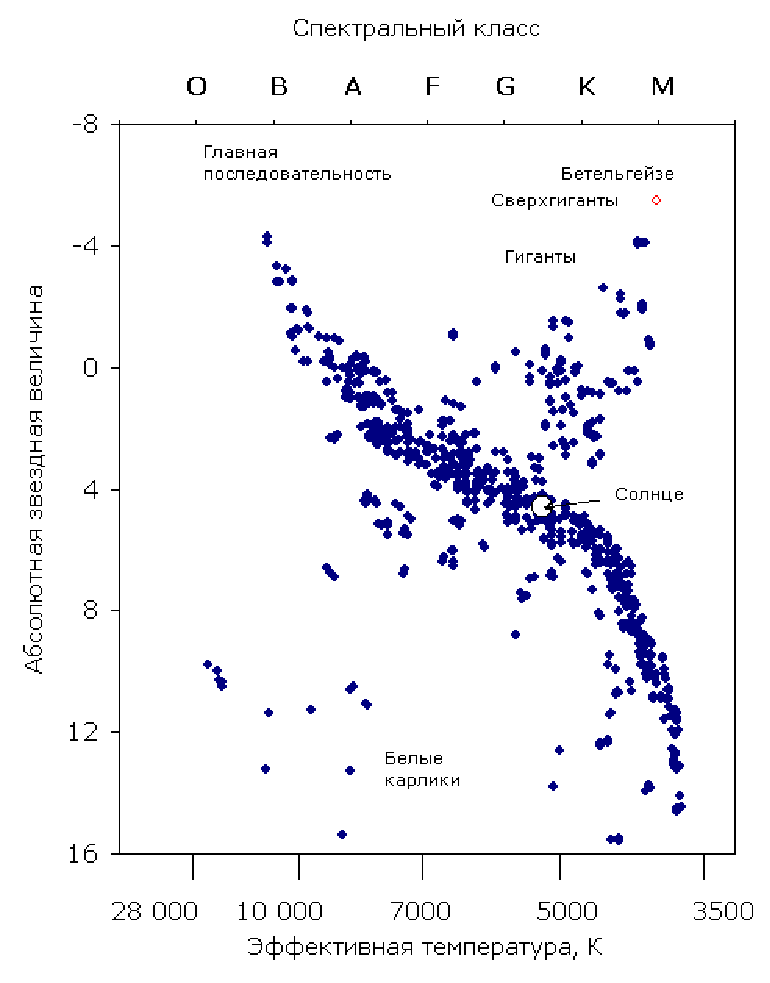
\includegraphics[scale=0.7]{spectr-typ}
\end{center}
\caption{Диаграмма Герцшпрунга-Рассела}
\end{figure}
\end{center}